\documentclass[@BEAMER_OPTIONS@]{beamer}
    @USE_PGFPAGES@

    \usetheme[alternativetitlepage=true,titleline=true]{Torino}
    \setbeamertemplate{navigation symbols}{}
    \setbeamertemplate{note page}[plain]

    \usepackage[utf8]{inputenc}
    \usepackage{graphicx}
    \usepackage{subfigure}
    \usepackage{xspace}
    \usepackage{adjustbox}
    \usepackage{tikz}
    \usepgflibrary{arrows}
    \usetikzlibrary{shadows,decorations.pathreplacing,patterns,shapes}
    \tikzstyle{every picture}=[semithick,>=stealth,remember picture]
    \usepackage{listings}
    \lstset{
        language=C++,
        basicstyle=\footnotesize\rmfamily,
        stringstyle=\color{chameleon4},
        numbers=left,
        numberstyle=\tiny,
        aboveskip=-0.02\baselineskip,
        belowskip=-0.02\baselineskip,
        columns=flexible,
        extendedchars=false,
        showstringspaces=false
        }
    \newcommand{\code}[1]{\lstinline|#1|}
    \newcommand{\additive}{\hspace{1cm}\footnotesize(\emph{Additive expressions only})}
    \newcommand{\Cpp}{{C\nolinebreak[4]\hspace{-.05em}\raisebox{.4ex}{\tiny\bf ++}}\xspace}
    \newcommand{\ghribbon}{
        \begin{tikzpicture}[remember picture,overlay]
            \node[anchor=north east,yshift=4pt,xshift=4pt] at (current page.north east) {
                \href{https://github.com/ddemidov/vexcl}{
\includegraphics[width=2cm]{forkme}}
            };
        \end{tikzpicture}
    }

    \title{VexCL -- Automatic OpenCL Code Generation}

    \author{Denis Demidov}
    \institute{
        Supercomputer Center of Russian Academy of Sciences \\
        Kazan Federal University
    }
    \date{October 2013, Austin, Texas}

\begin{document}

%----------------------------------------------------------------------------
\begin{frame}{}
    \titlepage
\end{frame}

\note{ }

%----------------------------------------------------------------------------
\begin{frame}{}
    \tableofcontents
\end{frame}

\note{ }

\section{Expression templates}

%----------------------------------------------------------------------------
\begin{frame}{Expression templates}
    \begin{itemize}
        \item How to implement a DSL in \Cpp \emph{effectively}?
            \vspace{\baselineskip}
        \item The idea is quite old:
            \begin{itemize}
                \item \emph{Todd Veldhuizen}, Expression templates, \Cpp Report,
                    \alert{1995}
            \end{itemize}
        \item First (?) implementation:
            \begin{itemize}
                \item Blitz++ \emph{is a \Cpp class library for scientific
                computing which provides performance\\
                on par with Fortran 77/90}.
            \end{itemize}
        \item Today:
            \begin{itemize}
                \item std::valarray, Boost.uBLAS, MTL, Eigen, Armadillo, etc.
            \end{itemize}
            \vspace{\baselineskip}
        \item<2> How does it work?
    \end{itemize}
\end{frame}

%----------------------------------------------------------------------------
\begin{frame}[fragile]{Simple example: Vector addition}
    \begin{exampleblock}{We want to be able to write:}
        \begin{lstlisting}
x = y + z;
        \end{lstlisting}
    \end{exampleblock}

    \begin{exampleblock}{And it has to be as effective as:}
        \begin{lstlisting}
for(size_t i = 0; i < n; ++i)
    x[i] = y[i] + z[i];
        \end{lstlisting}
    \end{exampleblock}
\end{frame}

%----------------------------------------------------------------------------
\begin{frame}[fragile]{\Cpp allows us to overload operators!}
    \begin{exampleblock}{}
        \begin{lstlisting}
const vector operator+(const vector &a, const vector &b) {
    assert(a.size() == b.size());
    vector c( a.size() );
    for(size_t i = 0; i < a.size(); ++i)
        c[i] = a[i] + b[i];
    return c;
}
        \end{lstlisting}
    \end{exampleblock}
    \begin{itemize}
        \item<2-> Any problems?
            \begin{itemize}
                \item<3-> Extra memory allocation
                \item<4-> Extra memory I/O
            \end{itemize}
    \end{itemize}
\end{frame}

%----------------------------------------------------------------------------
\begin{frame}[fragile]{Lazy evaluation v0.1}
    \begin{exampleblock}{}
        \begin{lstlisting}
struct vsum {
    const vector &a;
    const vector &b;
    vsum(const vector &a, const vector &b) : a(a), b(b) {}
};
        \end{lstlisting}
        \pause
        \begin{lstlisting}[firstnumber=last]

const vsum operator+(const vector &a, const vector &b) {
    return vsum(a, b);
}
        \end{lstlisting}
        \pause
        \begin{lstlisting}[firstnumber=last]

const vector& vector::operator=(const vsum &s) {
    for(size_t i = 0; i < data.size(); ++i)
        data[i] = s.a[i] + s.b[i];
    return *this;
}
        \end{lstlisting}
    \end{exampleblock}
\end{frame}

%----------------------------------------------------------------------------
\begin{frame}[fragile]{Lazy evaluation v0.1}
    \begin{exampleblock}{What happens if we write this?}
        \begin{lstlisting}
a = x + y + z;
        \end{lstlisting}
    \end{exampleblock}

    \begin{exampleblock}<2>{}
        \begin{verbatim}
lazy_v1.cpp:38:15: error: invalid operands to binary expression
      ('const vsum' and 'vector')
    a = x + y + z;
        ~~~~~ ^ ~
lazy_v1.cpp:12:12: note: candidate function not viable:
      no known conversion from 'const vsum'
      to 'const vector' for 1st argument
const vsum operator+(const vector &a, const vector &b) {
           ^
1 error generated.
        \end{verbatim}
    \end{exampleblock}
    \begin{description}
        \item<2>[Sidenote:] Clang error messages are awesome!
    \end{description}
\end{frame}

%----------------------------------------------------------------------------
\begin{frame}[fragile,shrink=2]{Lazy evaluation v0.2}
    \begin{exampleblock}{}
        \begin{lstlisting}
template <class LHS, class RHS>
struct vsum {
    const LHS &lhs;
    const RHS &rhs;
    vsum(const LHS &lhs, const RHS &rhs) : lhs(lhs), rhs(rhs) {}
    double operator[](size_t i) const {
        return lhs[i] + rhs[i];
    }
};
        \end{lstlisting}
        \pause
        \begin{lstlisting}[firstnumber=last]

template <class LHS, class RHS>
const vsum<LHS, RHS> operator+(const LHS &a, const RHS &b) {
    return vsum<LHS, RHS>(a, b);
}
        \end{lstlisting}
        \pause
        \begin{lstlisting}[firstnumber=last]

template<class Expr>
const vector& vector::operator=(const Expr &expr) {
    for(int i = 0; i < data.size(); ++i) data[i] = expr[i];
    return *this;
}
        \end{lstlisting}
    \end{exampleblock}
\end{frame}

%----------------------------------------------------------------------------
\begin{frame}{Last problem}
    \begin{itemize}
        \item There are times in life when addition alone is not enough\ldots
    \end{itemize}
\end{frame}

%----------------------------------------------------------------------------
\begin{frame}[fragile]{Lazy evaluation v0.3}
    \begin{exampleblock}{}
        \begin{lstlisting}
struct plus {
    static double apply(double a, double b) { return a + b; }
};
        \end{lstlisting}
        \pause
        \begin{lstlisting}[firstnumber=last]

template <class LHS, class OP, class RHS>
struct binary_op {
    const LHS &lhs;
    const RHS &rhs;
    binary_op(const LHS &lhs, const RHS &rhs) : lhs(lhs), rhs(rhs) {}
    double operator[](size_t i) const {
        return OP::apply(lhs[i], rhs[i]);
    }
};
        \end{lstlisting}
        \pause
        \begin{lstlisting}[firstnumber=last]

template <class LHS, class RHS>
const binary_op<LHS, plus, RHS> operator+(const LHS &a, const RHS &b) {
    return binary_op<LHS, plus, RHS>(a, b);
}
        \end{lstlisting}
    \end{exampleblock}
\end{frame}

%----------------------------------------------------------------------------
\begin{frame}[fragile]{Expression templates are trees}
    \begin{columns}
        \begin{column}{0.45\textwidth}
            \begin{exampleblock}{This expression:}
                \begin{onlyenv}<1>
                    \begin{lstlisting}[numbers=none]
x + y
                    \end{lstlisting}
                \end{onlyenv}
                \begin{onlyenv}<2>
                    \begin{lstlisting}[numbers=none]
x + y - z
                    \end{lstlisting}
                \end{onlyenv}
            \end{exampleblock}
            \begin{exampleblock}{... has this type:}
                \begin{uncoverenv}<2>
                    \begin{lstlisting}[numbers=none]
binary_op<
                    \end{lstlisting}
                \end{uncoverenv}
                \begin{lstlisting}[numbers=none]
    binary_op<
        vector,
        plus,
        vector
    >
                \end{lstlisting}
                \begin{uncoverenv}<2>
                    \begin{lstlisting}[numbers=none]
    , minus
    , vector
>
                    \end{lstlisting}
                \end{uncoverenv}
            \end{exampleblock}
        \end{column}
        \begin{column}{0.45\textwidth}
            \begin{figure}
                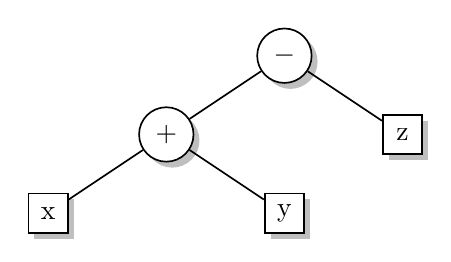
\begin{tikzpicture}
                    \uncover<2>{
                    \draw (0,0) node(sub)            [draw,fill=white,circle,drop shadow]{$-$};
                    \draw (sub) +( 1.50,-1) node(z)  [draw,fill=white,drop shadow,minimum size=0.5cm]{z};
                    }
                    \draw (sub) +(-1.50,-1) node(add)[draw,fill=white,circle,drop shadow]{$+$};
                    \draw (add) +(-1.50,-1) node(x)  [draw,fill=white,drop shadow,minimum size=0.5cm]{x};
                    \draw (add) +( 1.50,-1) node(y)  [draw,fill=white,drop shadow,minimum size=0.5cm]{y};

                    \uncover<2>{
                    \draw (sub) -- (add);
                    \draw (sub) -- (z);
                    }
                    \draw (add) -- (x);
                    \draw (add) -- (y);
                \end{tikzpicture}
            \end{figure}
        \end{column}
    \end{columns}
\end{frame}

%----------------------------------------------------------------------------
\begin{frame}[fragile]{So far, so good}
    \begin{exampleblock}{It is now possible to:}
        \begin{lstlisting}
v = a * x + b * y;

double c = (x + y)[42];
        \end{lstlisting}
    \end{exampleblock}

    \begin{exampleblock}{... and its as effective as:}
        \begin{lstlisting}
for(size_t i = 0; i < n; ++i)
    v[i] = a[i] * x[i] + b[i] * y[i];

double c = x[42] + y[42];
        \end{lstlisting}
    \end{exampleblock}
    \begin{itemize}
        \item No temporaries involved.
        \item Optimizing compiler is able to inline everything.
    \end{itemize}
\end{frame}

\section{OpenCL code generation}

\begin{frame}{}
    \tableofcontents[currentsection]
\end{frame}

%----------------------------------------------------------------------------
\begin{frame}{How does OpenCL work?}
    \begin{enumerate}
        \item A compute kernel is compiled at runtime from C99 source.
        \item Kernel parameters are set through API calls.
        \item Kernel is launched on a compute device.
    \end{enumerate}
    \vspace{\baselineskip}
    \pause
    \begin{itemize}
        \item Source may be read from a file, or stored in a static
            string, or \alert<2>{generated}.
    \end{itemize}
\end{frame}

%----------------------------------------------------------------------------
\begin{frame}[fragile]{Generating kernel source from an expression}
    \begin{exampleblock}{We want this expression:}
        \begin{lstlisting}
a = x + y - z
        \end{lstlisting}
    \end{exampleblock}
    \begin{exampleblock}{\ldots to result in this kernel:}
        \begin{lstlisting}
kernel void vexcl_vector_kernel(
    ulong n,
    global double * res,
    global double * prm1,
    global double * prm2,
    global double * prm3
)
{
    for(size_t idx = get_global_id(0); idx < n; idx += get_global_size(0)) {
        res[idx] = ( ( prm1[idx] + prm2[idx] ) - prm3[idx] );
    }
}
        \end{lstlisting}
    \end{exampleblock}
    \begin{tikzpicture}[overlay,scale=0.8]
        \draw (11,6) node(sub)[draw,fill=white,ellipse,drop shadow]{$-$};
        \draw (sub) +( 1.50,-1) node(z)  [draw,fill=white,drop shadow,minimum size=0.5cm]{z};
        \draw (sub) +(-1.50,-1) node(add)[draw,fill=white,circle,drop shadow]{$+$};
        \draw (add) +(-1.50,-1) node(x)  [draw,fill=white,drop shadow,minimum size=0.5cm]{x};
        \draw (add) +( 1.50,-1) node(y)  [draw,fill=white,drop shadow,minimum size=0.5cm]{y};
        \draw (sub) -- (add);
        \draw (sub) -- (z);
        \draw (add) -- (x);
        \draw (add) -- (y);
    \end{tikzpicture}
\end{frame}

%----------------------------------------------------------------------------
\begin{frame}[fragile]{Declaring parameters}
    \begin{exampleblock}{}
        \begin{lstlisting}
/*static*/ void vector::prm_decl(std::ostream &src, unsigned &pos) {
    src << ",\n    global double * prm" << ++pos;
}

template <class LHS, class OP, class RHS>
/*static*/ void binary_op<LHS, OP, RHS>::prm_decl(std::ostream &src, unsigned &pos) {
    LHS::prm_decl(src, pos);
    RHS::prm_decl(src, pos);
}
        \end{lstlisting}
    \end{exampleblock}
\end{frame}

%----------------------------------------------------------------------------
\begin{frame}[fragile]{Building expression string}
    \begin{exampleblock}{}
        \begin{lstlisting}
struct plus {
    static std::string string() { return "+"; }
};
        \end{lstlisting}
        \pause
        \begin{lstlisting}[firstnumber=last]

/*static*/ void vector::make_expr(std::ostream &src, unsigned &pos) {
    src << "prm" << ++pos << "[idx]";
}
        \end{lstlisting}
        \pause
        \begin{lstlisting}[firstnumber=last]

template <class LHS, class OP, class RHS>
/*static*/ void binary_op<LHS, OP, RHS>::make_expr(
                            std::ostream &src, unsigned &pos) const
{
    src << "( ";
    LHS::make_expr(src, pos);
    src << " " << OP::string() << " ";;
    RHS::make_expr(src, pos);
    src << " )";
}
        \end{lstlisting}
    \end{exampleblock}
\end{frame}

%----------------------------------------------------------------------------
\begin{frame}[fragile]{Source generation}
    \begin{exampleblock}{}
        \begin{lstlisting}
template <class Expr>
/*static*/ std::string vector::source() {
    std::ostringstream src; unsigned pos;

    src << "kernel void vexcl_vector_kernel(\n"
            "    ulong n,\n    global double * res";

    pos = 0; Expr::prm_decl(src, pos);

    src << ")\n{\n"
            "    for(size_t idx = get_global_id(0); idx < n; idx += get_global_size(0)) {\n"
            "        res[idx] = ";

    pos = 0; Expr::make_expr(src, pos);

    src << ";\n    }\n}\n";

    return src.str();
}
        \end{lstlisting}
    \end{exampleblock}
\end{frame}

%----------------------------------------------------------------------------
\begin{frame}[fragile]{Setting kernel arguments}
    \begin{exampleblock}{}
        \begin{lstlisting}
void vector::set_args(cl::Kernel &krn, unsigned &pos) {
    krn.setArg(pos++, buffer);
}

template <class LHS, class OP, class RHS>
void binary_op<LHS, OP, RHS>::set_args(cl::Kernel &krn, unsigned &pos) {
    lhs.set_args(krn, pos);
    rhs.set_args(krn, pos);
}
        \end{lstlisting}
    \end{exampleblock}
\end{frame}

%----------------------------------------------------------------------------
\begin{frame}[fragile]{Caching compiled kernels}
    \begin{itemize}
        \item Each kernel is uniquely identified by its expression type:
            \begin{itemize}
                \item Expression template captures terminal types and
                    operations.
            \end{itemize}
    \end{itemize}
    \begin{exampleblock}{}
        \begin{lstlisting}
template <class Expr>
const vector& vector::operator=(const Expr &expr) {
    static cl::Kernel kernel = build_kernel(device, source<Expr>());

    unsigned pos = 0;

    kernel.setArg(pos++, size);     // n
    kernel.setArg(pos++, buffer);   // res
    expr.set_args(kernel, pos);     // other parameters

    queue.enqueueNDRangeKernel(kernel, cl::NullRange, buffer.size(), cl::NullRange);

    return *this;
}
        \end{lstlisting}
    \end{exampleblock}
\end{frame}

\end{document}


% vim: et
